%------------------------------------------------------------------------
% Chapter:  Introduction
%------------------------------------------------------------------------

\chapter{Introduction \label{intro}}
\section{What is PDFFIT ?}

Now you might have installed {\it PDFFIT} and can start it simply
by typing {\tt pdffit} but in case you are not a PDF wizard here is
a little introduction into the PDF method first. For those who hate
to read long manuals, there is section \ref{quick} which shows how
to run a refinement in no time. The remaining users guide explains
the various features of {\it PDFFIT} more detail. \par

The determination of crystal structures is an important part of
chemistry, physics and of course crystallography. Conventional
structure determination is based on the analysis of the
intensities and positions of Bragg reflections which only allows
one to determine the long range {\it average} structure of the
crystal. Only one-body information such as atomic positions, site
occupancies and temperature factors can be extracted.
Determination of the {\it average} structure based on powder
diffraction data is now routinely done using the Rietveld
\citep{rietv;jac69} method which is very similar to the full
profile refinement of the atomic pair distribution function (PDF)
as we will see later. It should be kept in mind that the analysis
of Bragg scattering assumes a prefect long range periodicity of
the crystal. However, many materials are quite disordered and even
more important the key to the deeper understanding of their
properties is the study of deviations from the {\it average}
structure or the study of the {\it local} atomic arrangements.
Deviations from the {\it average} structure result in the
occurrence of diffuse scattering which contains information about
two-body interactions \citep{webu95,fr95}. In recent years the
analysis of diffuse scattering from single crystals as well as
powders using computer simulations have made great advances, in
particular using the Monte Carlo (MC) and the Reverse Monte Carlo
(RMC) technique \citep{webu95,nikemc95,wepr98,prwe98b,prwe97b}.
\par

Another method to reveal the {\it local} structure of a crystal is
the analysis of the PDF. This method is long known in the field of
studying short range order in liquids and glasses but has recently
been applied to crystalline materials \citep{egami;lsfd98,bieg93}.
The PDF is obtained from the powder diffraction data via a simple
Fourier transform of the normalised scattering intensity $S(Q)$:

\begin{equation}
  G(r) = 4 \pi r [ \rho(r) - \rho_{0} ] =
         \frac{2}{\pi} \int_{0}^{\infty} Q [S(Q) - 1] \sin(Qr) dQ,
  \label{eq_four}
\end{equation}

\noindent where $\rho(r)$ is the microscopic pair density,
$\rho_{0}$ is the average number density and $Q$ is the magnitude
of the scattering vector, for elastic scattering $Q=4\pi \sin
(\theta) / \lambda$ with $2\theta$ being the scattering angle and
$\lambda$ the wavelength of the radiation used. Details about the
determination of an experimental PDF can be found e.g. in
\citet{egami;lsfd98,warren} and are not discussed here. \par

Since the PDF contains Bragg and diffuse scattering, the
information about {\it local} arrangements is preserved. The PDF
can be understood as a bond-length distribution between all pairs
of atoms $i$ and $j$ within the crystal (up to a maximum
distance), however each contribution has a weight corresponding to
the scattering power of the two atoms involved as we will see a
little later. In order to carry out the Fourier transform in
(\ref{eq_four}) we would need to measure data up to $Q=\infty$,
which of course is not possible. Thus the termination at a value
of $Q=Q_{max}$ will cause so-called {\it termination ripples} in
the PDF. A short discussion of these {\it termination ripples} is
given in appendix \ref{app-deriv} or for a more detailed
discussion of the accuracy of PDF analysis see \citet{toeg92}.
With the availability of modern synchrotron and neutron sources it
is possible to collect powder diffraction data up to high values
in $Q$. \par

The study of a measured PDF ranges from a simple peak width
analysis revealing information about correlated motion
\citep{jeprmjbi98} to the full profile refinement of the PDF using
e.g. {\it PDFFIT} the manual of which you are currently reading.
In order to refine an experimental PDF one needs to calculate a
PDF from a structural model. This can be done using the relation

\begin{equation}
  G_{calc}(r) = \frac{1}{r} \sum_{i}\sum_{j} \left [
                \frac{b_{i}b_{j}}{\langle b \rangle ^{2}}
                \delta (r - r_{ij}) \right ]   - 4 \pi r \rho_{0},
  \label{eq_igr}
\end{equation}

\noindent
where the sum goes over all pairs of atoms $i$ and $j$ within the
model crystal separated by $r_{ij}$. The scattering power of atom $i$
is $b_{i}$ and $\langle b \rangle$ is the average scattering power
of the sample. In case of neutron scattering $b_{i}$ is simply the
scattering length, in case of X-rays it is the atomic form factor
evaluated at a user define value of $Q$ (set by the command {\tt xray}).
The default value is $Q=0$ in which case $b_{i}$ is simply the number
of electrons of atom $i$. Generally there are two different
ways to account for displacements (either thermal or static)
from the average position. First one can use a large enough model
containing the desired displacements and perform an ensemble average.
This is the method used by the program {\it DISCUS} where thermal
displacements can be introduced according to a given
(isotropic) Debye-Waller factor. Secondly one can convolute each
contribution given by $\delta (r - r_{ij})$ in (\ref{eq_igr}) with a
Gaussian accounting for the displacements (for details see appendix
\ref{app-deriv}). \par

Now we are ready for the first {\it PDFFIT} refinement example
presented in the next section. A detailed discussion about the
structural parameters that can be obtained and how they relate to
their 'long range' counterparts is given in section \ref{fit}.

%------------------------------------------------------------------------

\section{What is new ? \label{new}}

If you have used {\it PDFFIT} before, you might ask what is new in
this version of the program. Below you find sections describing the
major changes in the different releases of {\it PDFFIT}. A detailed
list of all changes can be found in the file {\it CHANGES.LOG} in
the source directory of the {\it PDFFIT} distribution.

\subsection*{Version 1.4}

This is the final release of {\it PDFFIT}. A completely redesigned
version is developed by the DANSE collaboration and more information
can be found in the paper by \cite{fajuli06}. New features in this
release os the support for spherical nano particles as well as the
introduction of named variables into the command language common for
all programs of the program package.

\begin{figure}[!t]
   \centering
   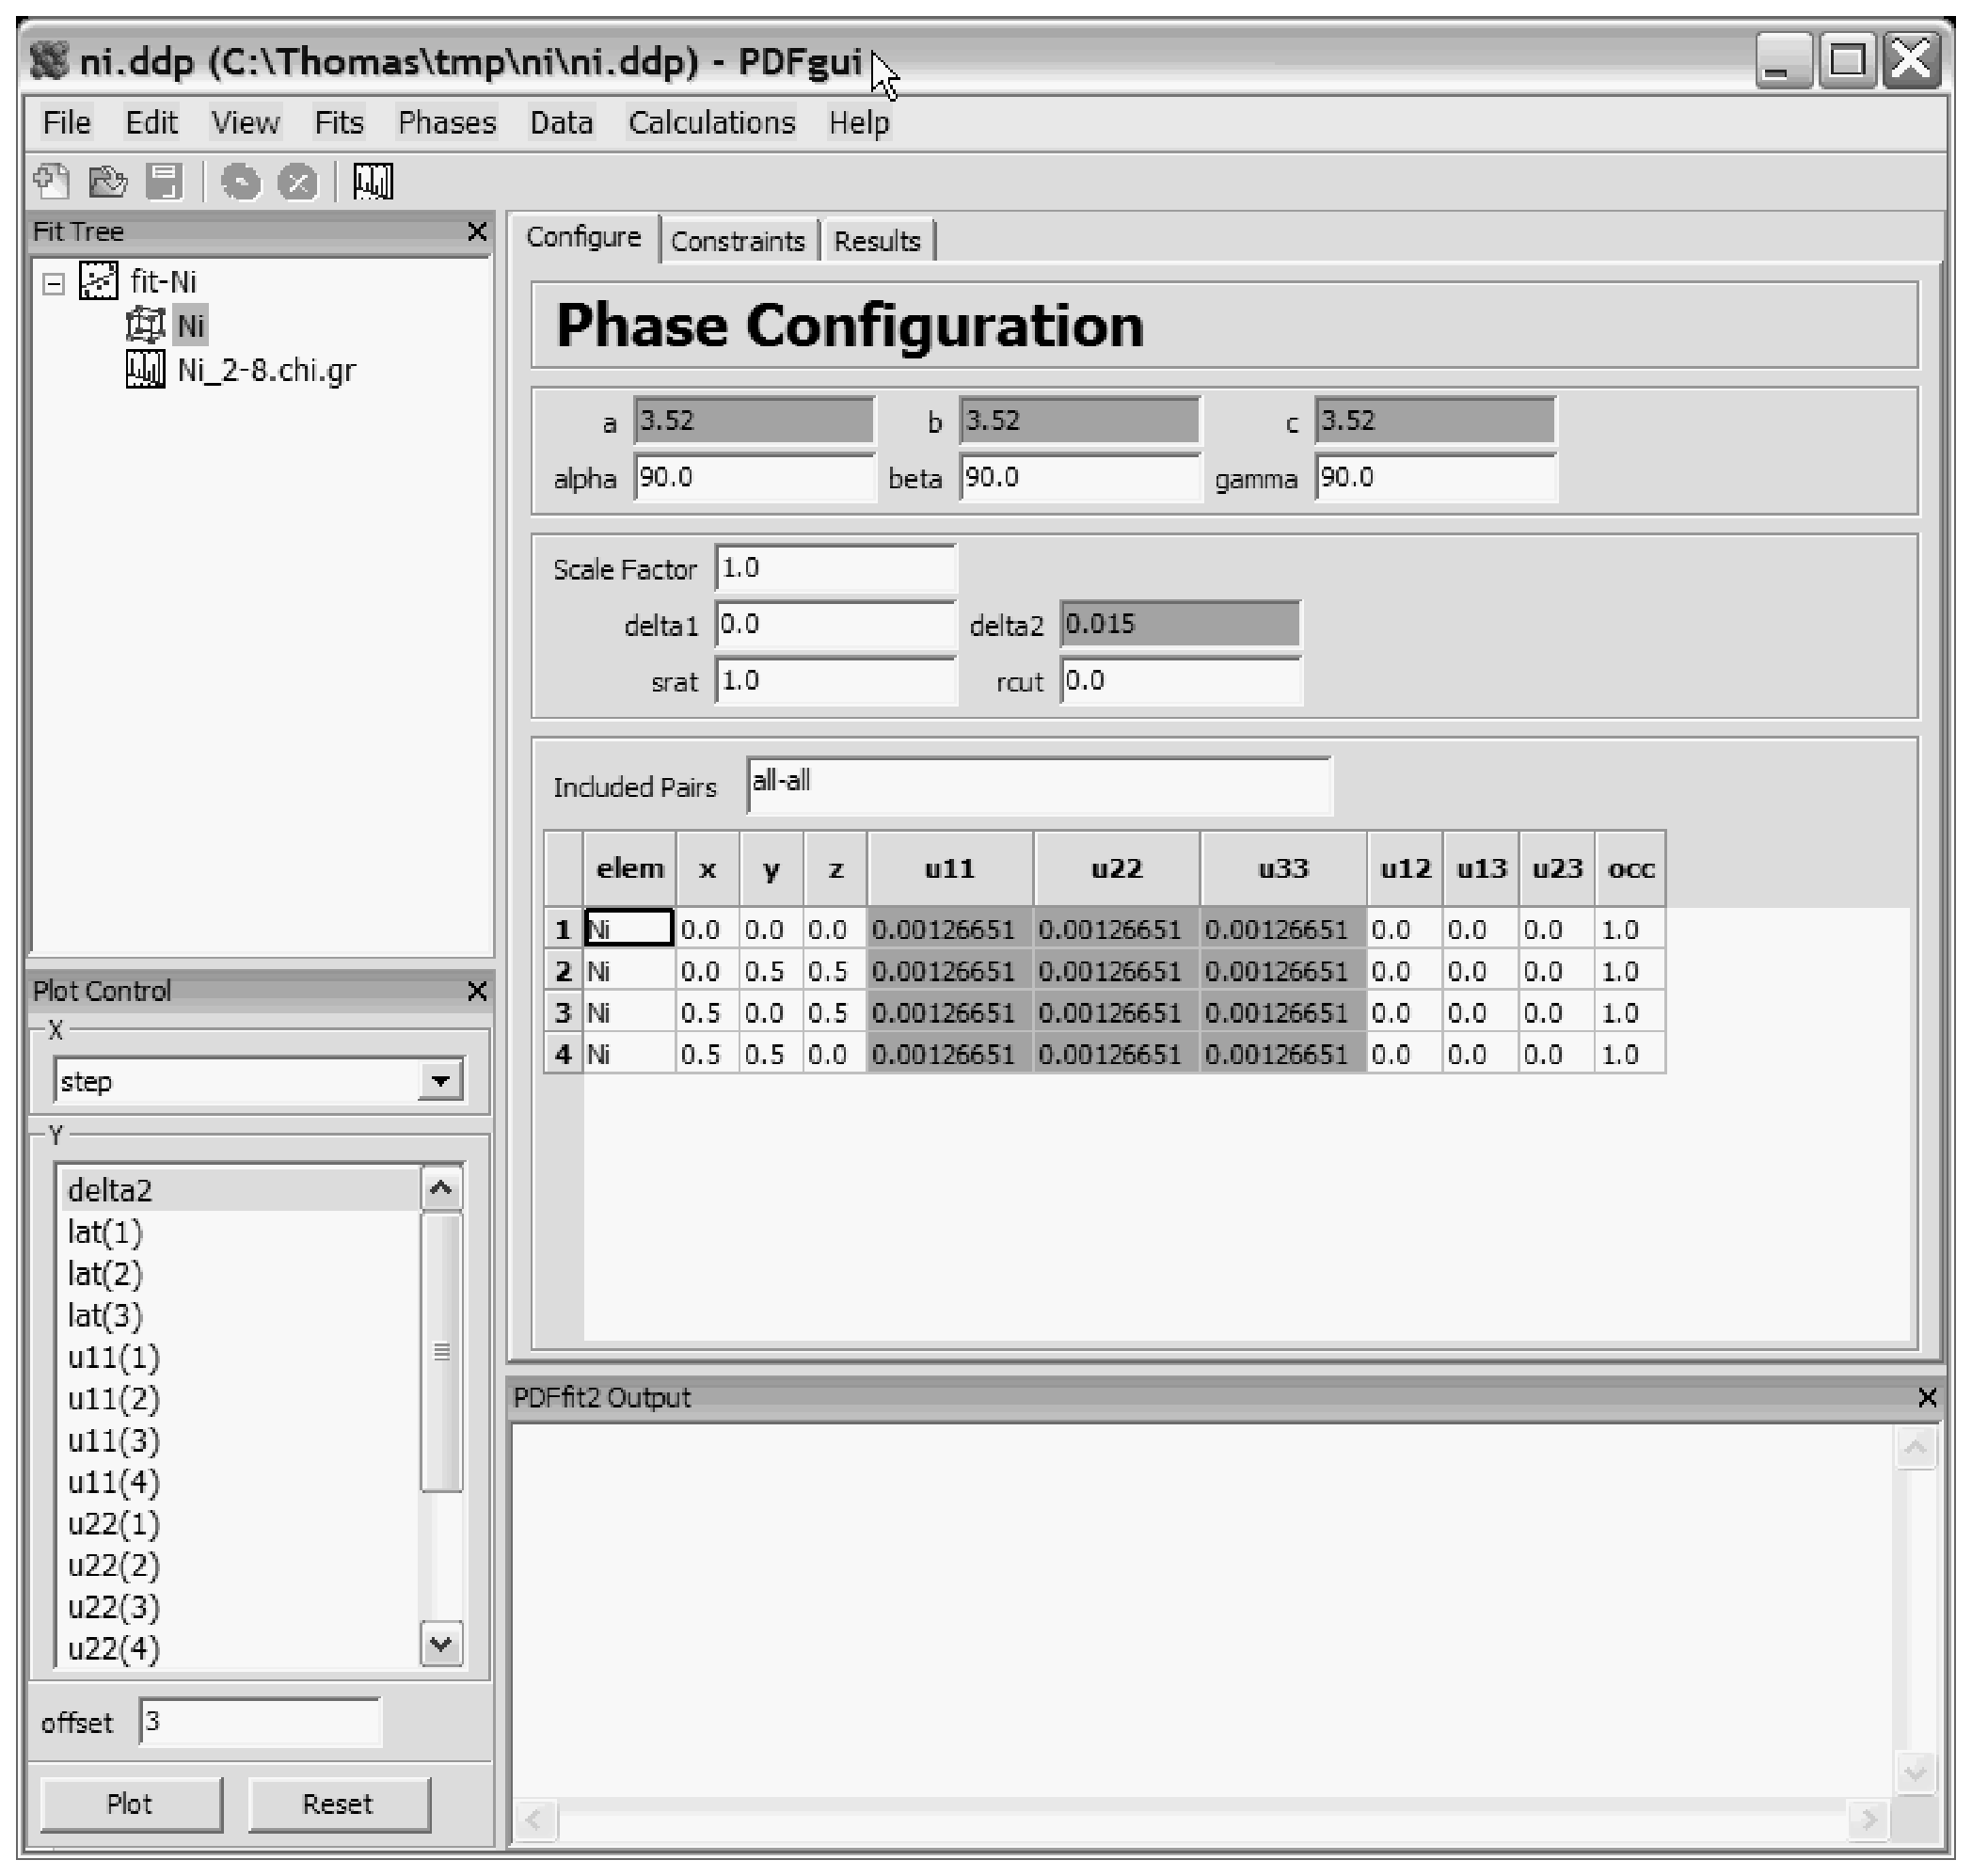
\includegraphics[width=2.5in, angle=0]{pdfnew.eps}
   \caption{Screen shot of beta version of next generation {\it PDFFIT}.}
\end{figure}


\subsection*{Version 1.3}

The main addition in this version are additional parameters to
control the PDF peak width. In addition to the quadratic term
variable, $\delta$, a linear correction has been added ($\gamma$).
In addition a PDF broadening correction determined by the instrument
resolution has been added ($\alpha$). For details on the new $r$
dependence of the PDF peak width refer to section \ref{fit_pwid}.
Following the work by \cite{thlele02}, the true PDF peak profile is
not purely a Gaussian. The corrected profile has now been
implemented in PDFFIT. Details can be found in Appendix
\ref{app-deriv}.

\subsection*{Version 1.2}

Besides various bug fixes, this new version of {\it PDFFIT} is now
distributed as self-extracting installer for the Windows operating
system. The program now supports system macros that can be
globally installed as well as reading macro files names from the
command line.

\subsection*{Version 1.1}

The following features were added to the program: {\it PDFFIT} is
now capable to export a structure in a format that can be read by
the program {\it ATOMS} \citep{prog;atoms} for 3D structural plots
(see section \ref{file_export}). The program now allows to refine
the difference between a PDF and a reference PDF. The command
language now includes simple commands for file input and output
(see section \ref{io}).

%------------------------------------------------------------------------

\section{Getting started \label{get}}

After the program {\it PDFFIT} is installed properly and the environment
variables are set, the program can be started by typing 'discus' at the
operating systems prompt. Information about the installation of {\it PDFFIT}
is given in appendix \ref{app-install}.

\begin{table}[!tbh]
\centering
\begin{tabularx}{\textwidth}{|p{30mm}|X|}
  \hline
  {\bf Symbol} & {\bf Description} \\
  \hline\hline
  "text"     &  Text given in double quotes is to be understood as typed. \\
  \hline
  $<$text$>$ &  Text given in angled brackets is to be replaced by an
                appropriate value, if the corresponding line is used
                in {\it PDFFIT}. It could, for example be the actual name
                of a file, or a numerical value. \\
  \hline
  {\tt text} &  Text in single quotes exclusively refers to {\it PDFFIT}
                commands. \\
  \hline
  $[$text$]$ &  Text in square brackets describes an optional parameter or
                command. If omitted, a default value is used, else
                the complete text given in the square brackets is to
                be typed. \\
  \hline
  \{text $|$ text\} &  Text given in curly brackets is a list of alternative
                parameters. A vertical line separates two alternative,
                mutually exclusive parameters. \\
  \hline
\end{tabularx}
\caption{\label{sym-tab}Used symbols}
\end{table}

The program uses a command language to interact with the user.  The
command {\tt exit} terminates the program and returns control to the
shell.  All commands of {\it PDFFIT} consist of a command verb,
optionally followed by one or more parameters.  All parameters must
be separated from one another by a comma ",".  There is no
predefined need for any specific sequence of commands.  {\it PDFFIT}
is case sensitive, all commands and alphabetic parameters MUST be
typed in lower case letters.  If {\it PDFFIT} has been compiled
using the {\tt -DREADLINE} option (see installation files) basic
line editing and recall of commands is possible.  For more
information refer to the reference manual or check the online help
using ('help command input').  Names of input or output files are to
be typed as they will be expected by the shell.  If necessary
include a path to the file.  All commands may be abbreviated to the
shortest unique possibility. At least a single space is needed
between the command verb and the first parameter.  No comma is to
precede the first parameter. A line can be marked as comment by
inserting a {\tt \#} as first character in the line.\par

The symbols used throughout this manual to describe commands,
command parameters, or explicit text used by the program {\it
PDFFIT} are listed in Table \ref{sym-tab}. There are several sources
of information, first {\it PDFFIT} has a build in online help, which
can be accessed by entering the command {\tt help} or if help for a
particular command $<$cmd$>$ is wanted by {\tt help $<$cmd$>$}. This
manual describes background and principle functions of {\it PDFFIT}
and should give some insight in the ways to use this program. \par

{\it PDFFIT} is distributed as part of the diffuse scattering
simulation software {\it DISCUS}.  However, {\it PDFFIT} can be used
as general plotting program separate from the {\it DISCUS} program
package.  To find out about recent updates of {\it PDFFIT} or to get
further information visit the {\it PDFFIT} WWW homepage:

\begin{center}
  {\it http://discus.sourceforge.net}
\end{center}

%------------------------------------------------------------------------
